\documentclass{article}
\usepackage{graphicx}
\usepackage{geometry}
\usepackage[MeX]{polski}
\usepackage[polish]{babel}
\usepackage{float}
\usepackage{fancyhdr}
\newcommand{\q}[1]{„#1“}
\usepackage{caption}
\usepackage{xcolor}
\usepackage[most]{tcolorbox}
\usepackage[scaled=0.85]{FiraMono} 

\usepackage[T1]{fontenc}
\usepackage{listings}
\usepackage[utf8]{inputenc}
\setlength{\parindent}{0pt} 

\newtcblisting{mylisting}{
arc=2mm,
top=0mm,
bottom=0mm,
left=3mm,
right=0mm,
boxrule=1pt,
colback=black!85,
listing only,
listing options={
basicstyle=\ttfamily\color{white},
showstringspaces=false,
language=Python,
keywordstyle=\color{myorange},
stringstyle=\color{mygreen},
commentstyle=\color{mygray}
xleftmargin=.2\textwidth, xrightmargin=.2\textwidth
}
}

\renewcommand{\labelenumii}{\arabic{enumi}.\arabic{enumii}}
\renewcommand{\labelenumiii}{\arabic{enumi}.\arabic{enumii}.\arabic{enumiii}}
\renewcommand{\labelenumiv}{\arabic{enumi}.\arabic{enumii}.\arabic{enumiii}.\arabic{enumiv}}

\definecolor{mygreen}{RGB}{26, 171, 26}
\definecolor{myorange}{RGB}{230,110,20}
\definecolor{mygray}{RGB}{100,100,100}


\tcbuselibrary{listings}

\begin{document}
\begin{center}\vspace{-1cm}
    \textbf{ \Huge Wykrywanie naczyń dna \\siatkówki oka}\\
    \LARGE Informatyka w medycynie\\
    \Large Zuzanna Cienka  \\
    \large nr albumu 148201\\
    \large \today \\~\\
\end{center}

\begin{enumerate}

    \item Zastosowany język programowania oraz dodatkowe biblioteki.
          \begin{itemize}
              \item Python
              \item OpenCV
              \item Numpy
              \item Matplotlib
          \end{itemize}
    \item Opis zastosowanych metod:
          \begin{enumerate}
              \item Przetwarzanie obrazów
              \begin{enumerate}
                \item Wstępne przetwarzanie obrazów\\
                Podczas wstępnego przetwarzania wyodrębniany jest kanał zielony, 
                następnie obraz jest rozmywany, a potem usuwany jest szum i przeprowadzane jest 
                wyostrzanie obrazu.
                \begin{figure}[h]
                    \centering
                    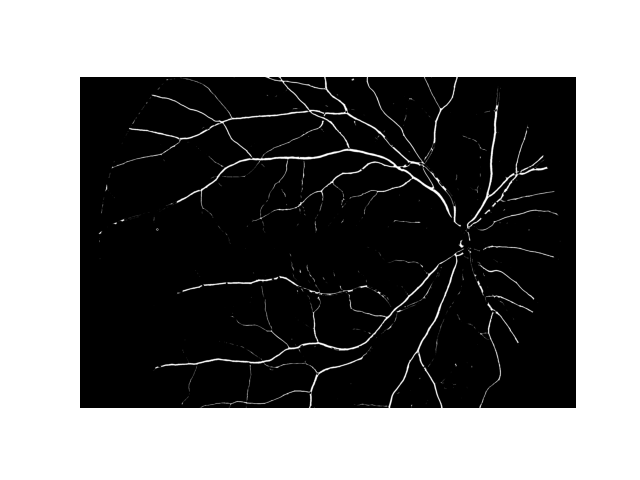
\includegraphics[width=0.6\textwidth]{../res/sample-preprocessed-image.png}
                    \caption{Obraz po wstępnym przetwarzaniu}
                  \end{figure}

              \end{enumerate}

          \end{enumerate}


\end{enumerate}

\end{document}
